\documentclass[12pt,letterpaper,noanswers]{exam}
\usepackage[usenames,dvipsnames,svgnames,table]{xcolor}
\usepackage[margin=0.9in]{geometry}
\renewcommand{\familydefault}{\sfdefault}
\usepackage{multicol}
\pagestyle{head}
\definecolor{c03}{HTML}{FFDDDD}
\header{AM 22b Class 13}{Updated \today.}{Feb 26: Skill Check}
\runningheadrule
\headrule
\usepackage{graphicx} % more modern
\usepackage{amsmath} 
\usepackage{amssymb} 
\usepackage{hyperref}
\usepackage{tcolorbox}


\newcommand{\mb}[1]{\underline{#1}}

\begin{document}
 \pdfpageheight 11in 
  \pdfpagewidth 8.5in

% Name: \rule{2.5in}{0.5pt}
% \vspace{4mm}


\begin{questions}
\item Let $D$ be the unit disk centered about the origin in $xy$-space.  Let $R$ be the right half of $D$.  Identify the sign of $\displaystyle\int_R 5y\ dA$.  Provide brief justification for your choice.
% \vfill

\begin{oneparcheckboxes}
\choice positive
\choice zero
\choice negative
\end{oneparcheckboxes}

\vfill

\item Reverse the order of integration for $\displaystyle\int_0^3\int_{x^2}^9 x\sin(y^2)\ dy\ dx$.  Do \textbf{not} evaluate the integral.

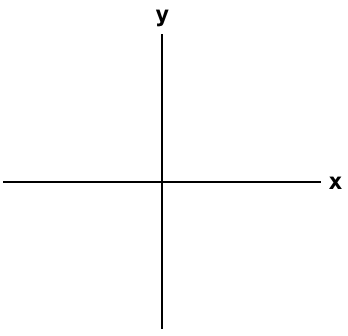
\includegraphics[height=2.5in]{img/C02axes-2.png}

\vfill

\end{questions}

\end{document}